
\clearpage









\section{Abstract}

The second chapter of my thesis.




%%%%%%%%%%%%%%%%%%%%%%%%%%%%%%%%%%%%%%%%%%%%%%%%%%%%%%%%%%%%%%%%%%%%%%%%%%%%%%%%%%%%%%%%%%%%%%%%%%%%%%%%%%%%%%%%%%%%%%%%%%%%%%%%%%%%%%%%%%%%%%%%%%%%%%%%%%%

\section{Introduction}

%%%%%%%%%%%%%%%%%%%%%%%%%%%%%%%%%%%%%%%%%%%%%%%%%%%%%%%%%%%%%%%%%%%%%%%%%%%%%%%%%%%%%%%%%%%%%%%%%%%%%%%%%%%%%%%%%%%%%%%%%%%%%%%%%%%%%%%%%%%%%%%%%%%%%%%%%%%

More text.


\section{Methods}

Here I describe my methods interspersed with the code that actually does it.











\begin{knitrout}\footnotesize
\definecolor{shadecolor}{rgb}{0.969, 0.969, 0.969}\color{fgcolor}\begin{figure}[t]

{\centering 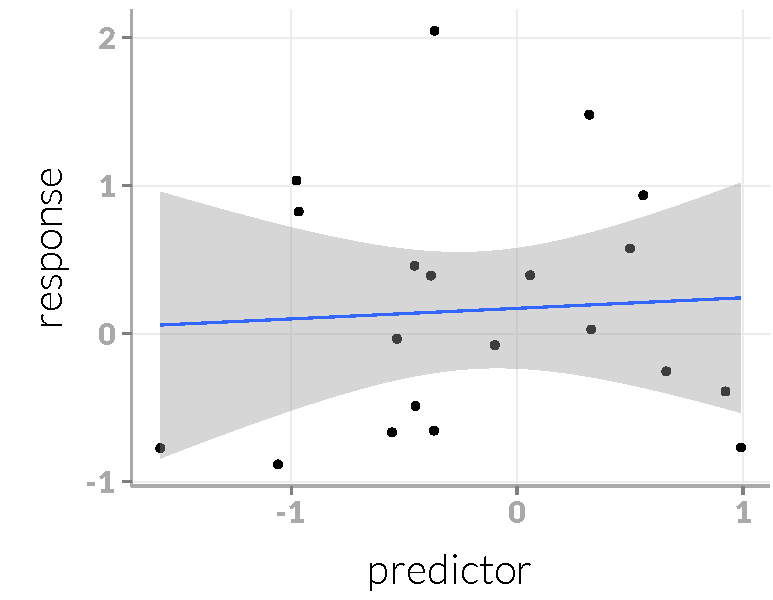
\includegraphics[width=0.8\textwidth]{figure/figPlots-1} 

}

\caption[A cruddy figure.]{
Caption labels can be really long so they might want to be separate. 
You can't have split lines in the knitr chunk options.
You figure legends should be version controlled too!
}\label{f:figPlots}
\end{figure}


\end{knitrout}

\section{Methods}

Remember to put results directly into text with \texttt{\\rinline}.
My model for this chapter isn't great (p = 0.8).

